\chapter{D-P~模型材料杆的有限元分析}
\label{cha:DP}
其他条件不变,将材料考虑为~D-P~硬化材料,假设内摩擦角为~{$10^\circ$},剪胀角为~{$10^\circ$},将模型材料进行调整,再进行有限元分析。圆杆~S33~应力云图、S23~应力云图和圆杆跨中截面正应力与剪应力分布云图如图~\ref{fig:dp}~所示。
\begin{figure}[htbp]
    \centering
	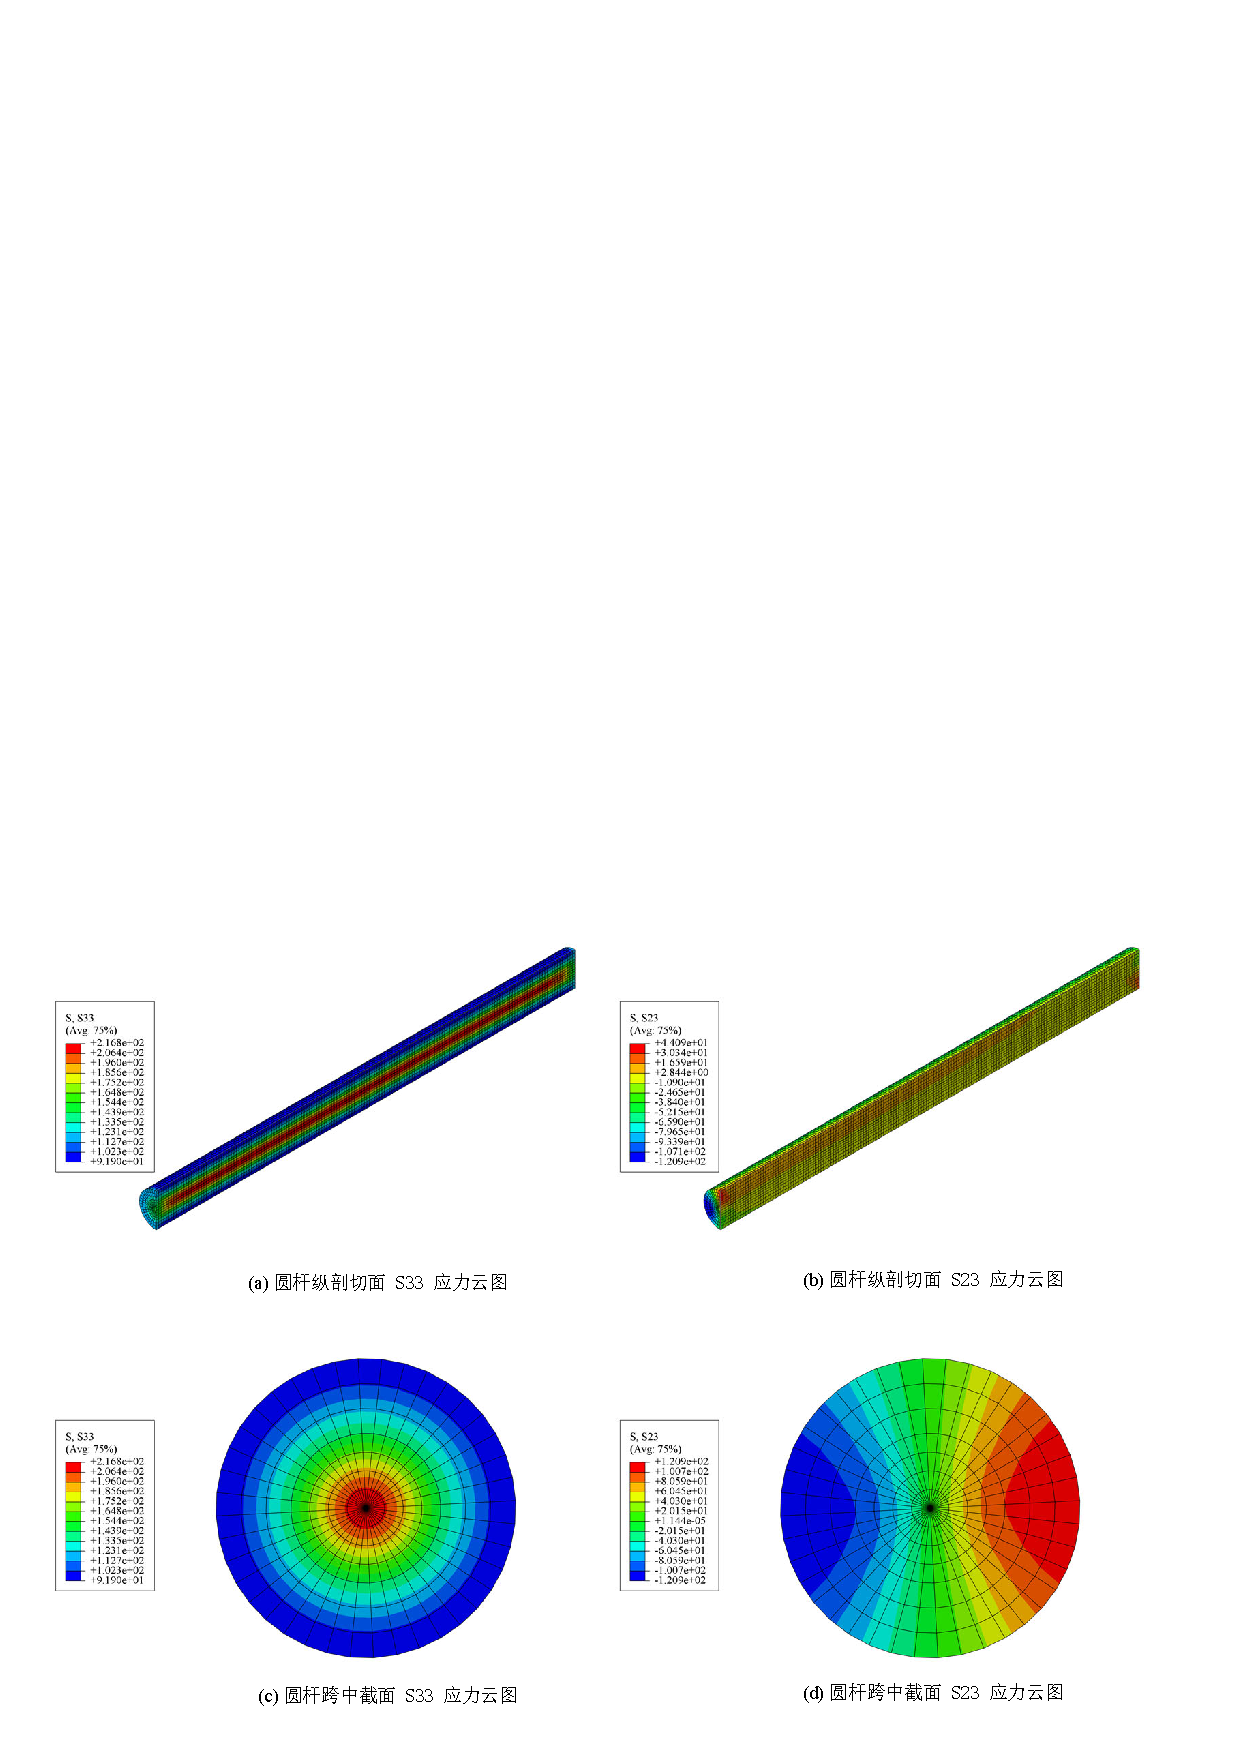
\includegraphics[width=1\textwidth]{dp.pdf}
    \caption{考虑~D-P~模型下圆杆数值模拟应力结果}
    \label{fig:dp}
\end{figure}

导出~D-P~模型材料条件下,圆杆跨中截面正应力与剪应力的径向分布结果,并与理想弹塑性材料、线性硬化材料条件下的有限元分析结果进行比较,绘制散点图如图~\ref{fig:dps3323}~所示。

观察曲线图可以发现,总体而言,三种材料条件下,圆杆跨中截面正应力和剪应力的分布符合相同趋势。D-P~模型下,截面正应力分布曲线接近理想弹塑性材料条件下的正应力分布曲线,截面剪应力分布曲线与线性硬化材料条件下的剪应力分布曲线较为吻合。

进一步总结可得,Drucker-Prager~准则更适用于描述那些有明显 体积效应或摩擦效应的材料。在该问题的分析中,使用~D-P~模型通常不会明显影响结果,因为钢材的屈服行为主要由剪应力决定,且其塑性硬化较为均匀。但在极端压力环境下(如在高压或大变形的情况下),D-P~模型可能会在一些特殊应用中提供更加精确的描述\cite{Drucker1952}。而~von Mises~准则更适合描述扭矩引起剪切应力下屈服等情况下的金属的塑性行为。
\begin{figure}[htbp]
    \centering
	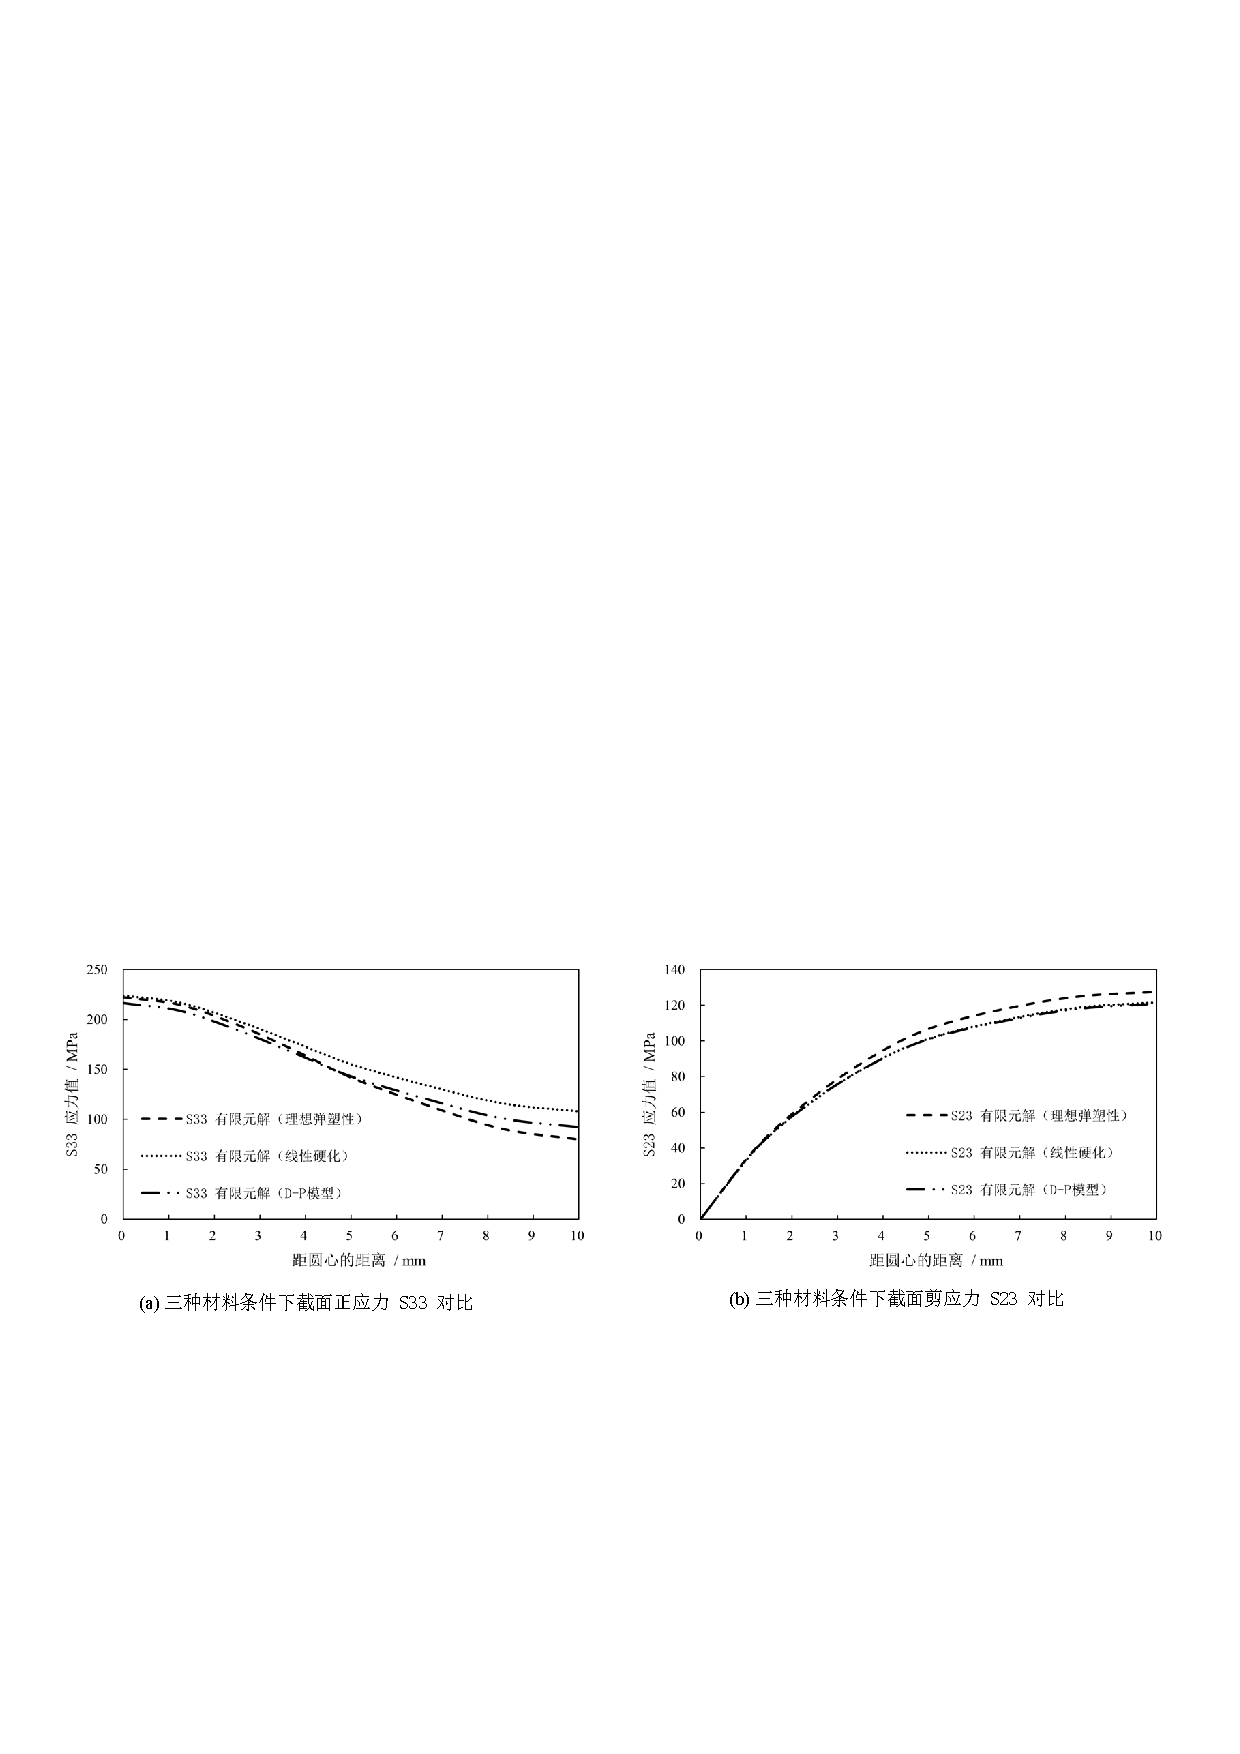
\includegraphics[width=1\textwidth]{3.pdf}
    \caption{三种材料条件下截面圆杆数值解对比}
    \label{fig:dps3323}
\end{figure}